\documentclass[onecolumn,10pt]{jhwhw}

\usepackage{algpseudocode}
\usepackage{amsfonts}
\usepackage{amsmath}
\usepackage{bm}
\usepackage{booktabs}
\usepackage{caption}
\usepackage{color}
\usepackage{commath}
\usepackage{empheq}
\usepackage{epsfig}
\usepackage{framed}
\usepackage{graphicx}
\usepackage{grffile}
\usepackage{listings}
\usepackage{mathtools}
\usepackage{pdfpages}
\usepackage{pgfplots}
\usepackage{siunitx}
\usepackage{wrapfig}

% Command "alignedbox{}{}" for a box within an align environment
% Source: http://www.latex-community.org/forum/viewtopic.php?f=46&t=8144
\newlength\dlf  % Define a new measure, dlf
\newcommand\alignedbox[2]{
% Argument #1 = before & if there were no box (lhs)
% Argument #2 = after & if there were no box (rhs)
&  % Alignment sign of the line
{
\settowidth\dlf{$\displaystyle #1$}
    % The width of \dlf is the width of the lhs, with a displaystyle font
\addtolength\dlf{\fboxsep+\fboxrule}
    % Add to it the distance to the box, and the width of the line of the box
\hspace{-\dlf}
    % Move everything dlf units to the left, so that & #1 #2 is aligned under #1 & #2
\boxed{#1 #2}
    % Put a box around lhs and rhs
}
}
% Default fixed font does not support bold face
\DeclareFixedFont{\ttb}{T1}{txtt}{bx}{n}{12} % for bold
\DeclareFixedFont{\ttm}{T1}{txtt}{m}{n}{12}  % for normal

\def\du#1{\underline{\underline{#1}}}

\author{John Karasinski}
\title{Homework \# 3}

\begin{document}
%\maketitle

\problem{}
Consider a robot manipulator as show in Figure P5.6. The kinematic structure of this robotic arm is very similar to that of the Stanford manipulator studied in example 5.6 except that it has an offset (a) between the base and the shoulder (the first two) join axes. For this robotic arm, derive and solve the kinematic position equations using shape and joint matrices.

There are two types of joints in this system, five revolute joints and one prismatic joint. Joints 1, 2, 4, 5, and 6 are revolute joints and have the following transformation matrix
\begin{align*}
\Phi_h (\phi_h) =
\begin{bmatrix*}[c]
\cos \phi_h & -\sin \phi_h & 0 & 0 \\
\sin \phi_h &  \cos \phi_h & 0 & 0 \\
          0 &            0 & 1 & 0 \\
          0 &            0 & 0 & 1 \\
\end{bmatrix*}
\end{align*}
Join 3 is a prismatic joint and has the following transformation matrix
\begin{align*}
\Phi_h (\phi_h) =
\begin{bmatrix*}[c]
          1 &            0 & 0 & \phi_h \\
          0 &            1 & 0 & 0 \\
          0 &            0 & 1 & 0 \\
          0 &            0 & 0 & 1 \\
\end{bmatrix*}
\end{align*}

\begin{figure}[h!]
  \centering
  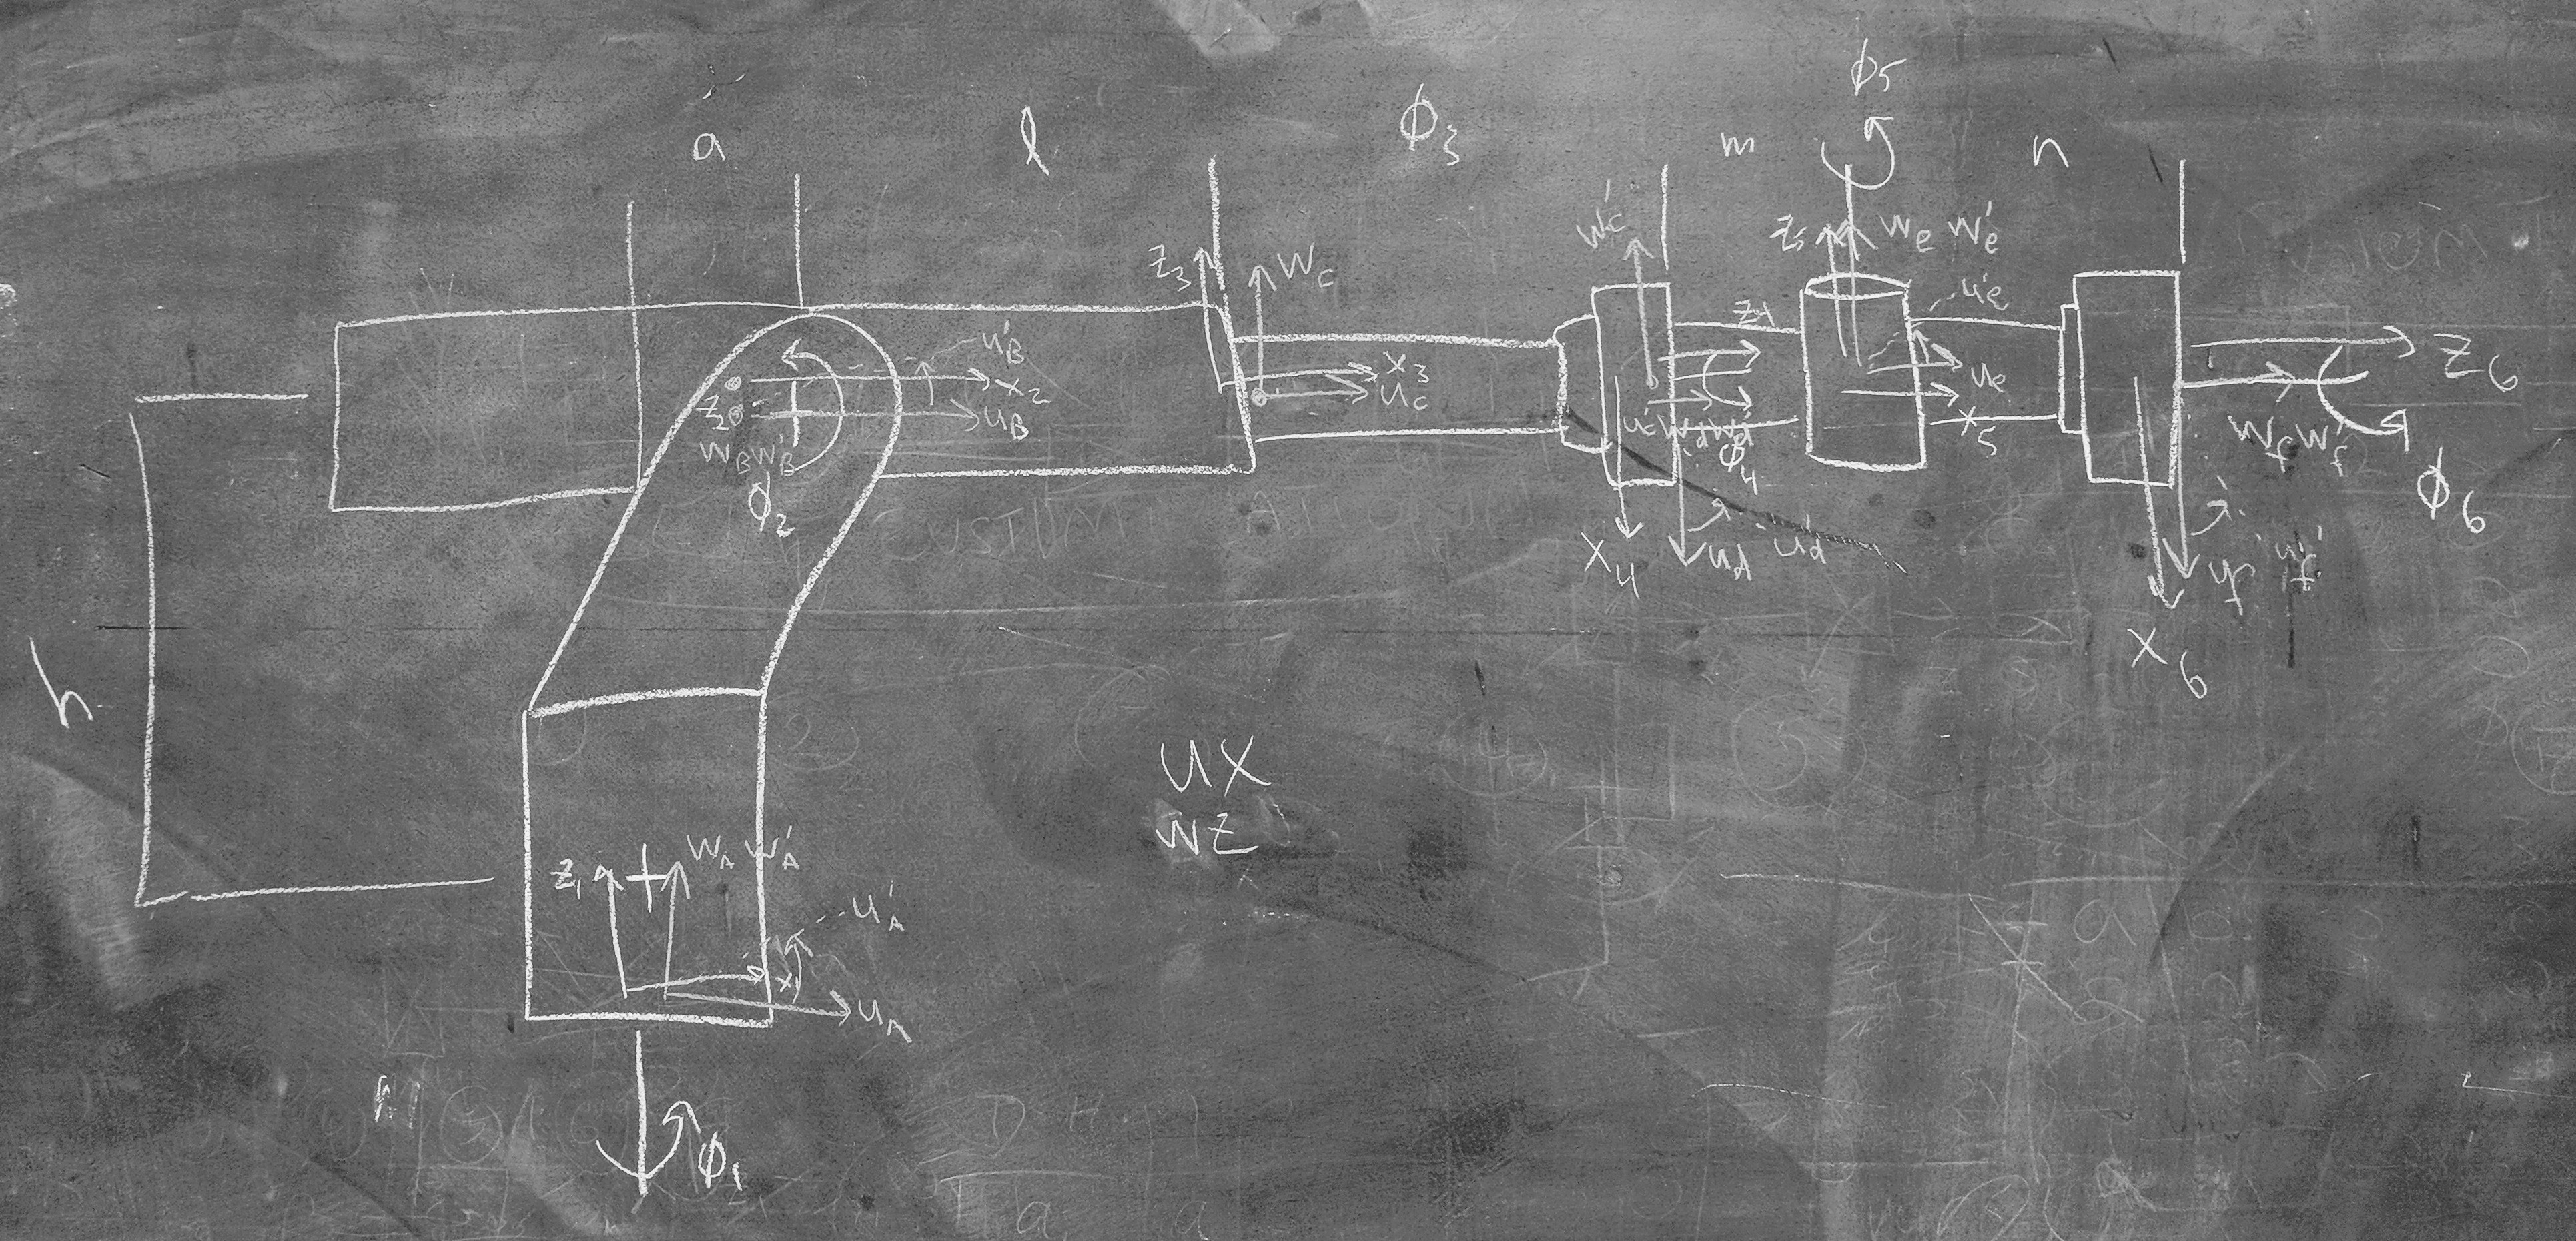
\includegraphics[width=\linewidth]{homework3-diagram.jpg}
  % \caption{}
  % \label{}
\end{figure}

Our shape matrices are obtained by inspection, and are

\begin{align*}
T_{01} & =
\begin{bmatrix*}[c]
 1 & 0 & 0 & x_0 \\
 0 & 1 & 0 & y_0 \\
 0 & 0 & 1 & z_0 \\
 0 & 0 & 0 & 1 \\
\end{bmatrix*}, \\
S_{1A} &= I, 
S_{2A} =
\begin{bmatrix*}[c]
1 & 0 & 0 & -a \\
0 & 0 & 1 & -h \\
0 & -1 & 0 & 0 \\
0 & 0 & 0 & 1 \\
\end{bmatrix*}, \\
S_{2B} &= I, 
S_{3B} = 
\begin{bmatrix*}[c]
1 & 0 & 0 & -l \\
0 & 0 & -1 & 0\\
0 & 1 & 0 & 0\\
0 & 0 & 0 & 1 \\
\end{bmatrix*}, \\
S_{3C} &= I, 
S_{4C} = 
\begin{bmatrix*}[c]
0 & 0 & -1 & 0 \\
0 & 1 & 0 & 0 \\
1 & 0 & 0 & 0 \\
0 & 0 & 0 & 1 \\
\end{bmatrix*}, \\
S_{4D} &= I, 
S_{5D} = 
\begin{bmatrix*}[c]
0 & 0 & 1 & -m \\
0 & 1 & 0 & 0 \\
-1 & 0 & 0 & 0 \\
0 & 0 & 0 & 1 \\
\end{bmatrix*}, \\
S_{5E} &= I, 
S_{6E} = 
\begin{bmatrix*}[c]
0 & 0 & -1 & 0 \\
0 & 1 & 0 & 0 \\
1 & 0 & 0 & -n \\
0 & 0 & 0 & 1 \\
\end{bmatrix*}, \\
S_{6F} &= I, 
S_{7F} = 
\begin{bmatrix*}[c]
-1 & 0 & 0 & 0 \\
0 & -1 & 0 & 0 \\
0 & 0 & 1 & 0 \\
0 & 0 & 0 & 1 \\
\end{bmatrix*}
\end{align*}

\begin{align*}
T_{i,i+1} &= S_{i, j} \Phi_j S_{i+1,j}^{-1} \\
T_{12} &= S_{1A} \Phi_A S_{2A}^{-1} \\
T_{23} &= S_{2B} \Phi_B S_{3B}^{-1} \\
T_{34} &= S_{3C} \Phi_C S_{4C}^{-1} \\
T_{45} &= S_{4D} \Phi_D S_{5D}^{-1} \\
T_{56} &= S_{5E} \Phi_E S_{6E}^{-1} \\
T_{67} &= S_{6F} \Phi_F S_{7F}^{-1} \\
\end{align*}

\begin{align*}
T_{12} &= S_{1A} \Phi_A S_{2A}^{-1} \\
&= I 
\begin{bmatrix*}[c]
\cos \phi_1 & -\sin \phi_1 & 0 & 0 \\
\sin \phi_1 &  \cos \phi_1 & 0 & 0 \\
          0 &            0 & 1 & 0 \\
          0 &            0 & 0 & 1 \\
\end{bmatrix*}
\begin{bmatrix*}[c]
1 & 0 & 0 & -a \\
0 & 0 & 1 & -h \\
0 & -1 & 0 & 0 \\
0 & 0 & 0 & 1 \\
\end{bmatrix*}^{-1} \\
&= 
\begin{bmatrix*}[c]
\cos \phi_1 & 0 &  \sin \phi_1 & a \cos \phi_1 \\
\sin \phi_1 & 0 & -\cos \phi_1 & a \sin \phi_1 \\
       0 & 1 &         0 &          h \\
       0 & 0 &         0 &          1 \\
\end{bmatrix*}
\end{align*}

\begin{align*}
T_{23} &= S_{2B} \Phi_B S_{3B}^{-1} \\
&= I 
\begin{bmatrix*}[c]
\cos \phi_2 & -\sin \phi_2 & 0 & 0 \\
\sin \phi_2 &  \cos \phi_2 & 0 & 0 \\
          0 &            0 & 1 & 0 \\
          0 &            0 & 0 & 1 \\
\end{bmatrix*}
\begin{bmatrix*}[c]
1 & 0 & 0 & -l \\
0 & 0 & -1 & 0 \\
0 & 1 & 0 & 0 \\
0 & 0 & 0 & 1 \\
\end{bmatrix*}^{-1} \\
&= 
\begin{bmatrix*}[c]
\cos \phi_2 &  0 & -\sin \phi_2 & l \cos \phi_2 \\
\sin \phi_2 &  0 &  \cos \phi_2 & l \sin \phi_2 \\
        0 & -1 &          0 &           0 \\
        0 &  0 &          0 &           1 \\
\end{bmatrix*}
\end{align*}

\begin{align*}
T_{34} &= S_{3C} \Phi_C S_{4C}^{-1} \\
&= I 
\begin{bmatrix*}[c]
          1 &            0 & 0 & \phi_3 \\
          0 &            1 & 0 & 0 \\
          0 &            0 & 1 & 0 \\
          0 &            0 & 0 & 1 \\
\end{bmatrix*}
\begin{bmatrix*}[c]
0 & 0 & -1 & 0 \\
0 & 1 & 0 & 0 \\
1 & 0 & 0 & 0 \\
0 & 0 & 0 & 1 \\
\end{bmatrix*}^{-1} \\
&= 
\begin{bmatrix*}[c]
0 &  0 & -1 & \phi_3 \\
0 &  1 &  0 &    0 \\
1 &  0 &  0 &    0 \\
0 &  0 &  0 &    1 \\
\end{bmatrix*}
\end{align*}

\begin{align*}
T_{45} &= S_{4D} \Phi_D S_{5D}^{-1} \\
&= I 
\begin{bmatrix*}[c]
\cos \phi_4 & -\sin \phi_4 & 0 & 0 \\
\sin \phi_4 &  \cos \phi_4 & 0 & 0 \\
          0 &            0 & 1 & 0 \\
          0 &            0 & 0 & 1 \\
\end{bmatrix*}
\begin{bmatrix*}[c]
0 & 0 & 1 & -m \\
0 & 1 & 0 & 0 \\
-1 & 0 & 0 & 0 \\
0 & 0 & 0 & 1 \\
\end{bmatrix*}^{-1} \\
&= 
\begin{bmatrix*}[c]
0 & -\sin \phi_4 & -\cos \phi_4 & 0 \\
0 &  \cos \phi_4 & -\sin \phi_4 & 0 \\
1 &          0 &          0 & m \\
0 &          0 &          0 & 1 \\
\end{bmatrix*}
\end{align*}

\begin{align*}
T_{56} &= S_{5E} \Phi_E S_{6E}^{-1} \\
&= I 
\begin{bmatrix*}[c]
\cos \phi_5 & -\sin \phi_5 & 0 & 0 \\
\sin \phi_5 &  \cos \phi_5 & 0 & 0 \\
          0 &            0 & 1 & 0 \\
          0 &            0 & 0 & 1 \\
\end{bmatrix*}
\begin{bmatrix*}[c]
0 & 0 & -1 & 0 \\
0 & 1 & 0 & 0 \\
1 & 0 & 0 & -n \\
0 & 0 & 0 & 1 \\
\end{bmatrix*}^{-1} \\
&= 
\begin{bmatrix*}[c]
 0 & -\sin \phi_5 & \cos \phi_5 & n \cos \phi_5 \\
 0 &  \cos \phi_5 & \sin \phi_5 & n \sin \phi_5 \\
-1 &          0 &         0 &           0 \\
 0 &          0 &         0 &           1 \\
\end{bmatrix*}
\end{align*}

\begin{align*}
T_{67} &= S_{6F} \Phi_F S_{7F}^{-1} \\
&= I 
\begin{bmatrix*}[c]
\cos \phi_6 & -\sin \phi_6 & 0 & 0 \\
\sin \phi_6 &  \cos \phi_6 & 0 & 0 \\
          0 &            0 & 1 & 0 \\
          0 &            0 & 0 & 1 \\
\end{bmatrix*}
\begin{bmatrix*}[c]
-1 & 0 & 0 & 0 \\
0 & -1 & 0 & 0 \\
0 & 0 & 1 & 0 \\
0 & 0 & 0 & 1 \\
\end{bmatrix*}^{-1} \\
&= 
\begin{bmatrix*}[c]
-\cos \phi_6 &  \sin \phi_6 & 0 & 0 \\
-\sin \phi_6 & -\cos \phi_6 & 0 & 0 \\
         0 &          0 & 1 & 0 \\
         0 &          0 & 0 & 1 \\
\end{bmatrix*}
\end{align*}
% From here the kinematic equations can be solved via
% \begin{align*}
% T_{23}^{-1} T_{12}^{-1} R_C &= T_{34} r_C^4 \\
% \begin{bmatrix*}[c]
%  X \cos \phi_1 \cos \phi_2 + Y \cos \phi_2 \sin \phi_1 + Z \sin \phi_2 - a \cos \phi_2 - h \sin \phi_2 - l \\
%                                                                             -X \sin \phi_1 + Y \cos \phi_1 \\
% -X \cos \phi_1 \sin \phi_2 - Y \sin \phi_1 \sin \phi_2 + Z \cos \phi_2 + a \sin \phi_2 - h \cos \phi_2     \\
%                                                                                                          1 \\
% \end{bmatrix*}
% &=
% \begin{bmatrix*}[c]
% \phi_3 \\
%    0 \\
%    0 \\
%    1 \\
% \end{bmatrix*} \\
% \end{align*}
% Solving the second row
% \begin{align*}
% 0 &= -X \sin \phi_1 + Y \cos \phi_1\\
% \tan \phi_1 &= \dfrac{Y}{X} \\
% \phi_1 &= \tan^{-1} \left ( \dfrac{Y}{X} \right )
% \end{align*}
% Solving for the third row
% \begin{align*}
% 0 &= \sin \phi_2 \left( -X \cos \phi_1 - Y \sin \phi_1 + a \right) + \cos \phi_2 \left( Z - h \right) \\
% -\sin \phi_2 \left( -X \cos \phi_1 - Y \sin \phi_1 + a \right)  &= \cos \phi_2 \left( Z - h \right) \\
% \tan \phi_2  &= \dfrac{-\left( Z - h \right)}{\left( -X \cos \phi_1 - Y \sin \phi_1 + a \right)} \\
% \phi_2  &= \tan^{-1} \left ( \dfrac{h - Z}{a -X \cos \phi_1 - Y \sin \phi_1 } \right ) \\
% \end{align*}
% Finally, the first line consists entirely of known variables
% \begin{align*}
% \phi_3 &= \cos \phi_2 \left ( X \cos \phi_1 + Y \sin \phi_1 - a \right) + \sin \phi_2 \left( Z - h \right) - l \\
% \end{align*}
From here the kinematic position can be solved via
\begin{align*}
R_C &= T_{12} T_{23} T_{34} r_C^4 \\
\begin{bmatrix*}[c]
x \\
y \\
z \\
1
\end{bmatrix*} &=
\begin{bmatrix*}[c]
a \cos\phi_1 + l \cos\phi_1 \cos\phi_2 + \phi_3 \cos\phi_1 \cos\phi_2 \\
a \sin\phi_1 + l \sin\phi_1 \cos\phi_2 + \phi_3 \sin\phi_1 \cos\phi_2 \\
                              h + l \sin\phi_2 + \phi_3 \sin\phi_2 \\
                                                             1 \\
\end{bmatrix*}
\end{align*}
where $r_C = \left[0, 0, 0, 1 \right]^T$.


% which results in the first three joint variables, $\phi_1, \phi_2,$ and $\phi_3$. The vectors $u_7^4, v_7^4,$ and $w_7^4$ can be calculated by
% \begin{align*}
% T_{56}^{-1} T_{45}^{-1} w_7^4 &= T_{67} w_7 \\
% \begin{bmatrix*}[c]
%                                                                                              w_7^{x_4} \cos \phi_4 + w_7^{y_4} \sin \phi_4 \\ 
% -w_7^{x_4} \cos \phi_5 \sin \phi_4 + w_7^{y_4} \cos \phi_4 \cos \phi_5 - w_7^{z_4} \sin \phi_5 + m \sin \phi_5 \\ 
%                                      -1-w_7^{x_4} \sin \phi_4 \sin \phi_5 + w_7^{y_4} \sin \phi_5 \cos \phi_4 + w_7^{z_4} \cos \phi_5 - m \cos \phi_5 - n \\
% 1 \\
% \end{bmatrix*}
% &= 
% \begin{bmatrix*}[c]
% 0 \\
% 0 \\
% 1 \\
% 0 \\
% \end{bmatrix*} \\
% \end{align*}
% which gives $w_7^{x_4}, w_7^{y_4},$ and $w_7^{x_4}$. The same can be done for the following equations
% \begin{align*}
% T_{56}^{-1} T_{45}^{-1} v_7^4 &= T_{67} v_7 \\
% T_{56}^{-1} T_{45}^{-1} u_7^4 &= T_{67} u_7 \\
% \end{align*}
% once these are found, the final $T_{17}$ can be built.



\problem{}
For the robot manipulator of problem 5.6, derive the kinematic position equations using Denavit-Hartenberg transformation matrices and find the solution to these equations using the partitioning method of section 5.7.

\begin{figure}[h!]
  \centering
  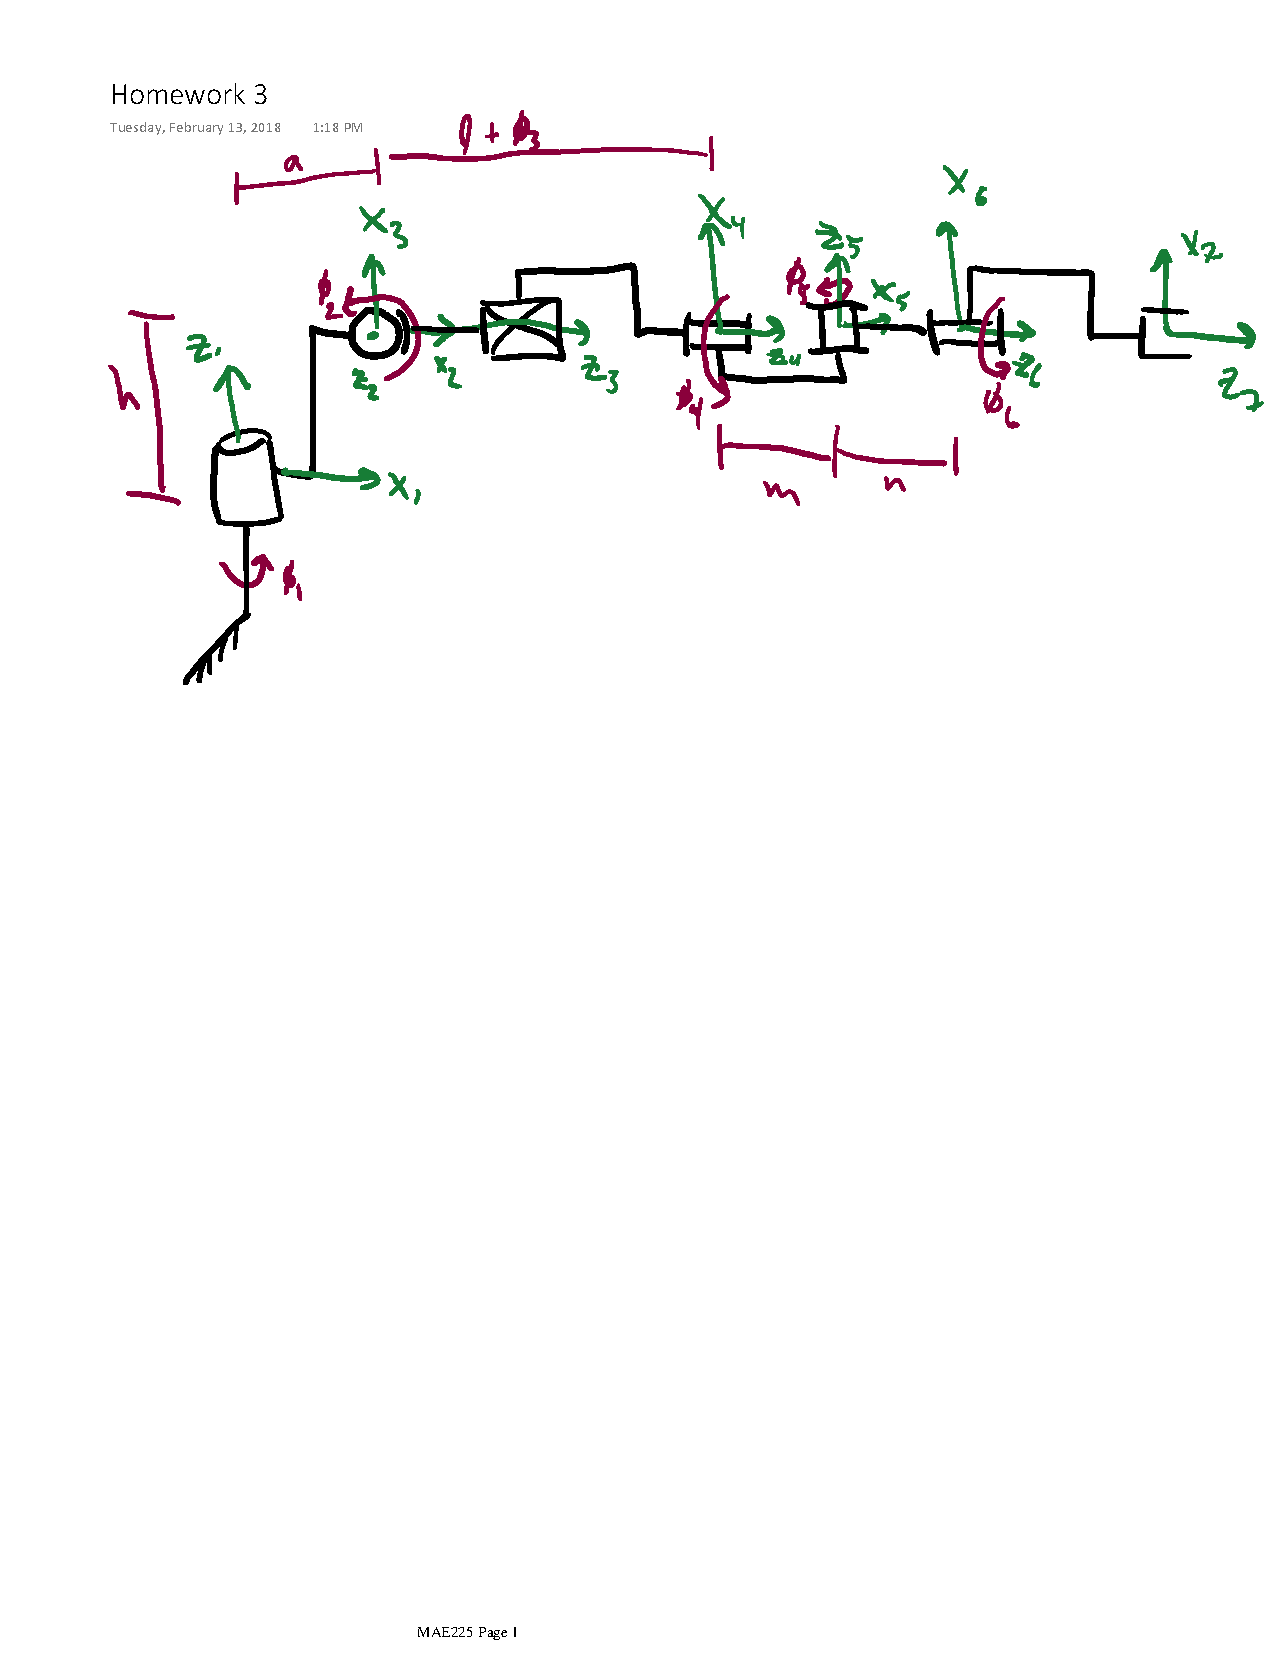
\includegraphics[width=\linewidth]{homework3-diagram.pdf}
  % \caption{}
  % \label{}
\end{figure}

\begin{center}
\begin{tabular}{r|rrrrrrr}
           & 1          & 2          & 3            & 4          & 5           & 6          \\
\midrule
$a_i$      & $a$        & 0          & 0            & 0          & 0           & 0          \\
$\alpha_i$ & $-\ang{90}$ & $\ang{90}$ & 0            & $\ang{90}$ & $\ang{-90}$ & $\ang{90}$ \\
$s_i$      & $h$        & 0          & $l + \phi_3$ & $m$        & $n$         & 0          \\
$\theta_i$ & $\phi_1$   & $\phi_2$   & 0            & $\phi_4$   & $\phi_5$    & $\phi_6$   \\
\end{tabular}
\end{center}

\begin{align*}
& T_1=
\begin{bmatrix*}[c]
\cos \phi_1 &  0 & -\sin \phi_1 & a \cos \phi_1 \\
\sin \phi_1 &  0 &  \cos \phi_1 & a \sin \phi_1 \\
          0 & -1 &          0 &           h \\
          0 &  0 &          0 &           1 \\
\end{bmatrix*},
& T_2=
\begin{bmatrix*}[c]
\cos \phi_2 & 0 &  \sin \phi_2 & 0 \\
\sin \phi_2 & 0 & -\cos \phi_2 & 0 \\
        0 & 1 &          0 & 0 \\
        0 & 0 &          0 & 1 \\
\end{bmatrix*}, \\
& T_3=
\begin{bmatrix*}[c]
1 & 0 & 0 &         0 \\
0 & 1 & 0 &         0 \\
0 & 0 & 1 & l + \phi_3\\
0 & 0 & 0 &         1 \\
\end{bmatrix*},
& T_4=
\begin{bmatrix*}[c]
\cos \phi_4 & 0 &  \sin \phi_4 & 0 \\
\sin \phi_4 & 0 & -\cos \phi_4 & 0 \\
        0 & 1 &          0 & m \\
        0 & 0 &          0 & 1 \\
\end{bmatrix*}, \\
& T_5=
\begin{bmatrix*}[c]
\cos \phi_5 &  0 & -\sin \phi_5 & 0 \\
\sin \phi_5 &  0 &  \cos \phi_5 & 0 \\
        0 & -1 &          0 & n \\
        0 &  0 &          0 & 1 \\
\end{bmatrix*},
& T_6=
\begin{bmatrix*}[c]
\cos \phi_6 & 0 &  \sin \phi_6 & 0 \\
\sin \phi_6 & 0 & -\cos \phi_6 & 0 \\
        0 & 1 &          0 & 0 \\
        0 & 0 &          0 & 1 \\
\end{bmatrix*}
\end{align*}

% \begin{align*}
% x_1 &= T_1 T_2 T_3 x_4 \\
% T_3^{-1} T_2^{-1} T_1^{-1} x_1 &= x_4 \\
% T_3^{-1} T_2^{-1} T_1^{-1} x_1 &=
% \begin{bmatrix*}[c]
% 0 \\
% 0 \\
% 0 \\
% 1
% \end{bmatrix*} \\
% \begin{bmatrix*}[c]
%  X \cos \phi_1 \cos \phi_2 + Y \sin \phi_1 \cos \phi_2 + Z \sin \phi_2 - a \cos \phi_2 - h \sin \phi_2  \\
%  X \sin \phi_1             - Y \cos \phi_1                                                              \\
%  X \cos \phi_1 \sin \phi_2 + Y \sin \phi_1 \sin \phi_2 - Z \cos \phi_2 - a \sin \phi_2 + h \cos \phi_2 - l + \phi_3 \\
% \end{bmatrix*}
% &=
% \begin{bmatrix*}[c]
% 0 \\
% 0 \\
% 0 \\
% \end{bmatrix*} \\
% \mbox{Further,}\\
% x_4 &= T_4 T_5 T_6 x_7
% \begin{bmatrix*}[c]
% 0 \\
% 0 \\
% 0 \\
% 1
% \end{bmatrix*} \\
% &= T_4 T_5 T_6 x_7 \\
% \begin{bmatrix*}[c]
% X (-\sin \phi_4 \sin \phi_6  + \cos \phi_4 \cos \phi_5 \cos \phi_6 ) - Y \sin \phi_5 \cos \phi_4  + Z (\sin \phi_4 \cos \phi_6  + \sin \phi_6 \cos \phi_4 \cos \phi_5 ) + n \sin \phi_4 \\
% X (\sin \phi_4 \cos \phi_5 \cos \phi_6  + \sin \phi_6 \cos \phi_4 )  - Y \sin \phi_4 \sin \phi_5  + Z (\sin \phi_4 \sin \phi_6 \cos \phi_5  - \cos \phi_4 \cos \phi_6 ) - n \cos \phi_4 \\
% X \sin \phi_5 \cos \phi_6                                            + Y \cos \phi_5              + Z \sin \phi_5 \sin \phi_6  + m \\
% \end{bmatrix*} \\
% \end{align*}


\end{document}
